\chapter{現地の生活や文化の紹介}
本章ではインドでの生活や休日の旅行を通して思ったことを中心に記載する。
\section{平日の様子}
%\begin{wrapfigure}{r}{0.5\textwidth}
%\vspace*{-\intextsep}
%  \begin{center}
%    \includegraphics[width=0.5\textwidth]{pic/wtc.eps}
%    \caption{\acrshort{wtc}}
%    \label{wtc}
%  \end{center}
%\vspace*{-6\intextsep}
%\end{wrapfigure}
筆者が滞在したホテルは\acrshort{hil}オフィスが入居する\acrlong{wtc}から南に5km下った場所にあった。
\acrshort{wtc}とホテル間の移動にはホテル手配の車を利用した。
バスまたはメトロと徒歩で通勤することも可能であったが、\acrshort{hil}の方針で駐在員は研修員含めて仕事関係の移動は全て車を使うこととなっていた。
\acrshort{wtc}には\acrshort{ama}社のオフィスも入居しており、ホテルからの行き帰りの車で\acrshort{ama}社員と同乗することがよくあった。
話をすると、彼らは新しく\acrshort{ama}に採用されて一時的にホテルに滞在しているとのことである場合が多かった。
複数の\acrshort{ama}社員が同乗した場合は、おそらく機密事項に当たるであろうことを人のすぐ隣で大声で情報交換していた。
\par
出勤では当初ホテルを午前8時に出発していた。しかしある日突然\acrshort{wtc}へのメインロードが工事を開始したため通勤路を迂回しなければならなくなり、
ホテルを出る時間を早めなければならなくなった。
その工事は来る日も来る日も一切進んでいる気配がなく、遂に数ヶ月経って筆者が帰国する日になっても地面に大きな穴が空いたままであった。
\par
ホテルや\acrshort{wtc}、メトロの駅やショッピングモールの入り口では荷物検査と簡単なボディ検査が実施されている。
しかし職員の動きを見ている限りではそれはあくまでも形式上のもので、とても本当の危険物を発見できる体制には思えなかった。
建物内にはいたるところに警備員が配置されていた。
しかし一見過剰に思える人員配置や諸々の複雑な手続きも、それらの仕事によって雇用が確保されているので、無駄を省き全体の効率を図ろうとする力学がインド社会ではなかなか成立しないようである。
\par
\acrshort{hil}の終業時刻は午後5時であり、職場のほとんど全てのインド人が定時で帰宅していた。
筆者は日本にいた頃は慢性的に残業をしていたが、\acrshort{hil}は定時で帰るのが当たり前の環境であることと、ホテルの車に予め帰りの時間を指定していることで
筆者もほぼ定時で帰るようになった。
それに自然と仕事のリズムも合うようになり、定時でキリが良いように仕事が進むようになってそれで業務にも全く支障がなかった。
日本に帰っても無駄に残業せずに、基本的に定時で帰る前提で仕事を進めることを継続したい。
\begin{figure}[ht]
  \begin{minipage}{0.5\hsize}
  \begin{center}
    \includegraphics[width=\textwidth]{pic/wtc.eps}
  \end{center}
%   \caption{\acrshort{wtc}}
%   \label{orggraph}
  \end{minipage}
  \begin{minipage}{0.5\hsize}
  \begin{center}
    \includegraphics[width=\textwidth]{pic/cow.eps}
  \end{center}
%   \caption{適用後(85ノード、123エッジ)}
%   \label{minigraph}
  \end{minipage}
  \caption{\acrshort{wtc}とインドの道路。だいたい100m間隔で牛に遭遇する。}
  \label{wtc}
\end{figure}
%\begin{figure}[ht]
%  \centering
%  \includegraphics[width=0.7\textwidth]{pic/wtc.eps}
%  \caption{\acrlong{wtc}}
%  \label{wtc}
%\end{figure}
%\subsection{ホテル}
%\subsection{移動}
%\subsection{職場}
\section{週末の様子}
日本でやっていたテニスを継続したいと思いバンガロールで練習できる環境を探したところ、インド人ローカルのテニスクラブと日本人会のテニス部を見つけて毎週練習をしていた。
平日の移動手段が全て車であり日常生活で運動する機会がホテルのジム以外になかったため、週末のテニスは体力を維持するためにもとても助けになった。
ローカルのテニスクラブはコーチとの1対1レッスンで1時間Rs.600($\simeq$ \yen1000)と言われ、
インド人感覚からするとほぼぼったくり価格であったが、日本でスクールに通うよりはいくらか安いため
承知の上で月に一回くらい練習をさせてもらっていた。
コーチは毎週毎週「今週末は来るのか?」と電話をかけてくる非常に営業熱心な19歳の青年であった。
\par
日本人会テニス部では政府関係の人や企業の駐在員とその家族また学生までが一緒に練習していて、バンガロールに暮らしているたくさんの日本人と知り合うことができた。
活動場所はホテルから約4km離れた公園(Cubbon Park)内にある\acrshort{kslta}スタジアムであった。
ここではプロの試合も行われることがあり、2015年10月には\acrshort{kslta}で行われたATPチャレンジャーツアー男子ダブルスの決勝を観戦した。
練習日時は金曜日18:30-20:30と日曜日10:00-13:00であった。
夜に練習する場合は停電があると照明が復旧するまで15分ほど中断してしまうことや、コートが別の予定で突然使えなくなるなど、不便はあったものの
日本にいたときよりもはるかにたくさん練習を積むことができていろいろなショットが打てるようになった。
そのほかには平日の定時後にコンドミニアム敷地内にあるコートで練習することもあった。
\begin{figure}[ht]
  \begin{minipage}{0.5\hsize}
  \begin{center}
    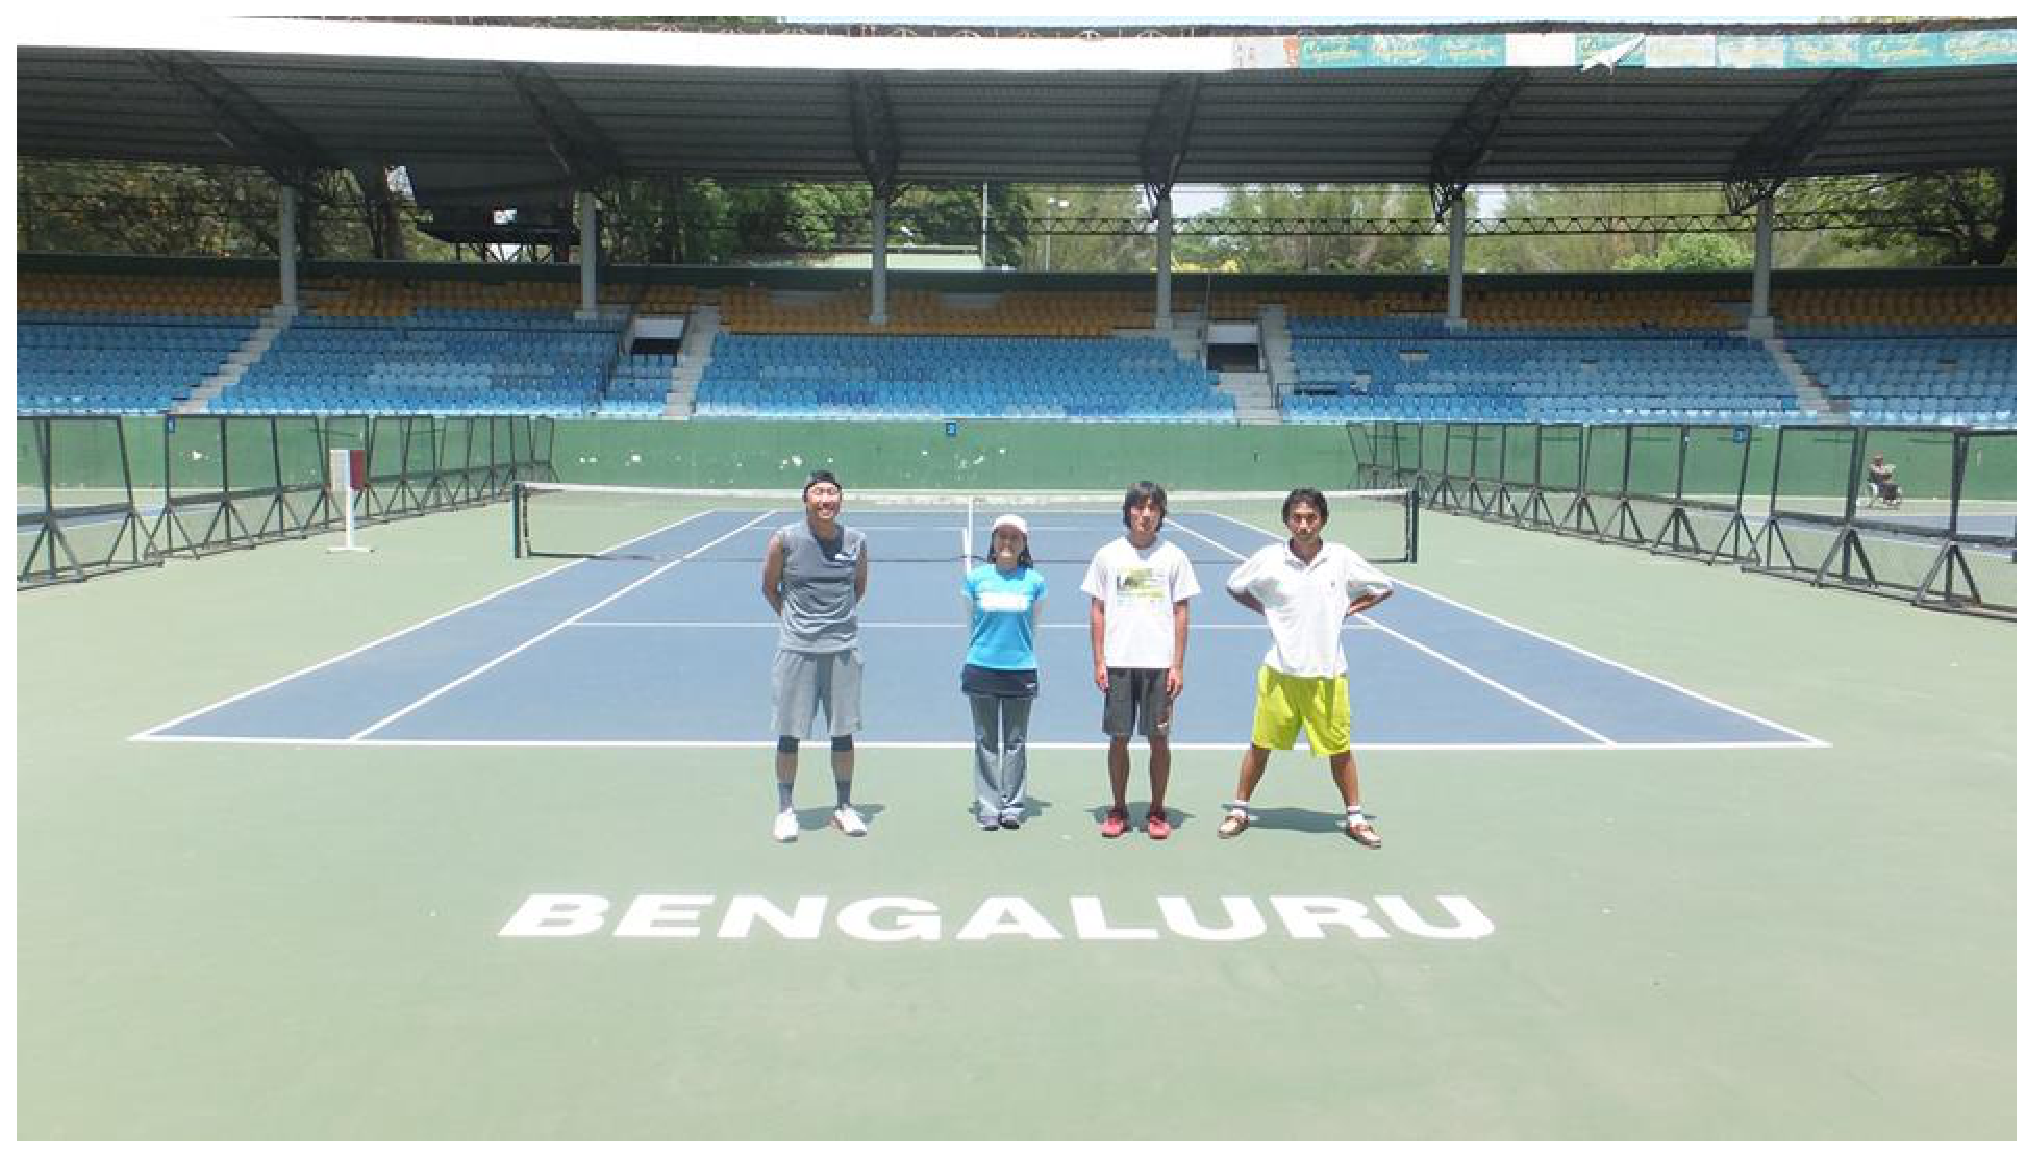
\includegraphics[width=\textwidth]{pic/kslta.eps}
  \end{center}
  \end{minipage}
  \begin{minipage}{0.5\hsize}
  \begin{center}
    \includegraphics[width=\textwidth]{pic/local.eps}
  \end{center}
  \end{minipage}
  \caption{\acrshort{kslta}スタジアムとインド人テニスクラブ。「今週は行けない」と言っても何度も電話してくる。}
  \label{wtc}
\end{figure}
\par
日曜日の夕方には\href{https://www.facebook.com/jinseidojo/timeline}{\acrlong{toast}} \cite{toast}に参加することがあった。
\acrshort{toastint} \cite{toastint}はパブリックスピーチや話し方の上達を目的とする国際的な団体で、バンガロールのコミュニティでは
日本語の勉強をしているインド人と英語の勉強をしている日本人が一緒に活動をしていた。
活動はバイリンガルで行われていて互いに言語の教え合いをすることもあった。
筆者は\acrshort{hil}の駐在員に紹介してもらって参加した。
即興で話題を振られて何かを話したり、即興で物語を作ったり、即興で他人のスピーチの論評したりと、とても頭を使う活動であった。
\begin{figure}[ht]
  \begin{minipage}{0.65\hsize}
  \begin{center}
    \includegraphics[width=\textwidth]{pic/toast1.eps}
  \end{center}
  \end{minipage}
  \begin{minipage}{0.35\hsize}
  \begin{center}
    \includegraphics[width=0.9\textwidth]{pic/toast2.eps}
  \end{center}
  \end{minipage}
  \caption{\acrshort{toast}バンガロールコミュニティ。筆者よりも日本語の語彙が豊富なインド人がいる。}
  \label{toast}
\end{figure}
\section{交通事情}
インドで暮らす上で、日本と全く異なるインドの交通事情に適応することは避けて通れない。
タクシーだけではなく様々な乗り物を使えるようになれば行動範囲と自由度がとても広がる。
本節では各交通手段別にそれぞれの特徴を述べる。
\subsection{バス}
筆者は休日に移動する際はほとんどバスを使用していた。
しかし筆者が聞いた限り、周りの日本人でバンガロールのバスに乗ったことのある人はいなかった。
それは、たくさんのバスが街中を走っている中で乗る場所や乗り方また行き先が分からないからである。
\acrshort{hil}のインド人に聞いてもバンガロールのバスは複雑でしかも不安定なので普通使わないと言っていた。
\par
バンガロールには100を超える数の路線バスが走っている。それぞれ、V-335EV, 258CC, KBS-3Eのような
数字とアルファベットの組み合わせが路線名としてバスの先頭に表示されている。
路線名の表示は手書きだったり、電光であっても消えていたり、現地語で書かれたりするため、まず路線名の視認が困難なことが多い。
路線名は走る地域や行き先によって似たような数字が割り当てられているようであるが、その規則性は全く不明である。
乗るべき路線名はGoogle Mapで行き先を調べることで分かるものの時間は全く当てにできない。
Google Mapでは通常複数の路線名が検索結果に出てくるので、それらを全てメモしておくとバスに乗れる確率が高まる。
なぜなら、Google Mapで示されたバス停に行っても狙った路線名のバスが一定時間内に来るとは限らないからである。
バス停といっても時刻表やバス停名などといった親切なものは一切なく、かろうじて屋根と椅子があることでバス停と分かるものとなっている。
目印が全くなく人が集まっているだけのバス停もある。
特に僻地のバス停ほどバスが来る頻度が低いため、乗ることのできる路線名をできる限り多く把握しておくことが必要となる。
筆者の場合はホテルから徒歩15分程度の場所にバンガロールシティ駅に隣接するバスターミナル(Kempegowda Bus Station)があったので、
バスの乗り降りはそのバスターミナルで行った。ここでは近辺の全ての路線が乗り入れるので、乗りたい路線にほぼ確実に一定時間内に乗ることができた。
\par
バスの料金は、乗ってからしばらくしてやってくる集金係に行き先を告げると金額を教えてくれるので手渡しで支払う。
親切な集金係だと伝えた場所に着くと知らせてくれる場合もあるが、基本的に自分で降りる場所を把握していなければならない。
気の利いた車内アナウンスなどはもちろんない。
料金は5km-15kmの道のりでだいたいRs.10-20($\simeq$ \yen15-30)と非常に安い。
ここでRs.50紙幣やRs.100紙幣を出すと受け取ってもらえないか非常に嫌がられるので、Rs.1やRs.10単位の細かい額を持っておかないと支払いに手間取ってしまう。
Rs.500紙幣やRs.1000紙幣などは言語道断である。どうしても集金係にお釣りがないときは、
「降りるときに何ルピー受け取る」というメモをその場で書いて渡してくれる。
もちろん申告しなかったり降りるときもお釣りがなかったりという場合はもらうことができない。
バスに限らず商店やモールでもみんなが細かいお金を欲しがるので、気をつけて小額紙幣や小銭を切らさないようにしていないとRs.500札やRs.1000札だけになってしまい
日常生活に支障をきたすことになる。
\par
バスには必ず運転手と集金係の必ず二人のスタッフがいる。
バスがどんなにぎゅうぎゅう詰めに混んでいても、集金係は新しく乗ってきた人を見失わずに人を押し退けバスの中を前に後ろに移動するのでとても大変である。
バスの中は前半分が女性で後半分が男性の空間という暗黙の了解があり、空いているからといって前に座ると注意される。
バスは走行中もドアが常に開きっぱなしで、ドアが壊れていることもよくある。バス車体の状態は整備という概念があるのか疑問に思うほどで、どのバスもひどい排気ガスを放出していた。
道路が平らでないことも相まって乗り心地は良いとは言えないが、タイミングよく乗ることができれば非常に安価で便利な移動手段である。
ただし道路が渋滞しているときは徒歩よりも遅い。
\begin{figure}[ht]
  \begin{minipage}{0.5\hsize}
  \begin{center}
    \includegraphics[width=\textwidth]{pic/busint.eps}
  \end{center}
  \end{minipage}
  \begin{minipage}{0.5\hsize}
  \begin{center}
    \includegraphics[width=\textwidth]{pic/kbs.eps}
  \end{center}
  \end{minipage}
  \caption{バンガロール市内の路線バス内とKempegowda Bus Station内の案内の一つ}
  \label{bus}
\end{figure}
\subsection{鉄道}
インドの鉄道には主に都市間や長距離を結ぶディーゼル機関車と、デリーなどの都市圏内で運行するメトロと言われる電車がある。
ここでは中長距離を結ぶ\acrlong{ir}について記載する。
筆者は週末や休日の旅行の際に\acrlong{ir}を利用した。インド滞在中に利用した区間は
Mumbai-Aurangabad間(約360km、8時間)、Bangalore-Mysore間(約140km、3時間)、Bangalore-Hospet間(約350km、8時間)
であった。
\acrlong{ir}を利用するためには座席の予約が必要であることになっている。
ただし後述するように事実上は予約せず運賃も払わずに乗車することは可能であるため、
無賃乗車で利用している客は一定数存在すると思われる。
筆者は\acrshort{maketrip}というインドの旅行手配サービス\cite{maketrip}を日本人会テニス部で教えてもらい、そこを介して\acrlong{ir}チケットの購入を行った。
駅の窓口で直接チケットを購入することもできるようであるが、\acrlong{ir}の座席予約システムが非常に複雑であることもあり
インド人と直接会話してチケットを確実に確保できる自信がなかったためweb上で予約を行った。
\par
\acrlong{ir}チケットを購入するためには、前提として\acrshort{wl}という\acrlong{ir}独自のシステムを理解する必要がある。
\acrlong{ir}にはこの複雑な\acrshort{wl}システムに起因する数々の独自のしきたりが存在しており、
特に旅行者が\acrlong{ir}を利用する際に混乱する要因となっている。
web上を検索するとこの\acrlong{ir}予約方法に関する\acrshort{wl}用語の質問や解説が山のように出てくるほか、
\href{http://trainstuff.in/}{\acrlong{ir}の利用方法ノウハウを第三者がまとめたサイト} \cite{trainstuff}
では\acrshort{wl}の仕組み解説のために特別にページを割いているほどである。
大前提として、\acrlong{ir}チケットは購入した時点で座席が確保されない。
座席数を超える予約が入っている場合であっても\acrlong{ir}予約システム上はチケットを購入できてしまうため、
それをもって実際に座席を確保できる条件を予め把握しておかないと、
予約が確定したと勘違いした結果当日になって列車に乗ることが出来ないということが起こり得る。
\par
用意された座席数が埋まっていない場合は座席の権利が確定したチケット(confirmed)を購入できるが、
既に埋まっている場合は\gls{rac}または\acrshort{wl}と呼ばれる区分のチケットを購入することになる。
\acrshort{rac}は「列車に乗車する権利があるが座席は保証しない」チケットである。
この場合は座席の権利を持った客が現れない場合そこに座るか、他の客の席を分けてもらうか、または立って乗車することになる。
confirmedチケットのキャンセルがあると随時先着順で\acrshort{rac}がconfirmedに繰り上がる。
confirmedと\acrshort{rac}で割当てられた分のチケットが売り切れると\acrshort{wl}チケットを購入することとなる。
\acrshort{wl}は座席の権利も乗車の権利もなにもなく、
confirmedチケットまたはRACチケットでキャンセルがあることを前提に権利が繰り上がることが期待できるのみである。
当日になっても\acrshort{wl}から繰り上がらなかった場合は料金が自動的に返金される。
\acrshort{rac}または\acrshort{wl}は購入する時点で何人たまっているのかが分かるようになっており、
購入した後もキャンセル状況によって自分がリストの何番目なのかの情報が\acrshort{maketrip}サイト上で随時更新されるため、
乗車・座席の権利が繰り上がる可能性をある程度予測することができる。
\acrshort{wl}チケットはさらに4種類ほどのタイプに区分されるがここではこれ以上の説明を省略する。
どの区分のチケットであっても期日前なら特にペナルティなくキャンセルが可能である。
ただし\acrshort{maketrip}や\acrlong{ir}のサイトは特に夜間不安定になる傾向があるため、
予約手続きが途中で失敗したりサイトが一時閉鎖していたりということに頻繁に遭遇する。
\acrshort{wl}の仕組みを理解し、かつ\acrshort{maketrip}上の手続きが成功して初めて何らかの乗車可能性が期待できるチケットを購入することができる。
\par
当日になってconfirmedチケットを手にしていた場合であっても座席の場所は
列車の発車時刻数時間前に用意されるChartを確認するまで把握することが出来ない。
Chartはその列車に乗車できる客の最終確定リストであって、乗車直前に\acrshort{maketrip}で確認するか、
駅の端末または張り出された紙で確認するか、各車両のドアに張り出された紙を確認する必要がある。
Chartには客の名前や性別年齢等の個人情報がプライバシー無関係に記載されている。
当日になってChartに自分の名前があることと座席番号が記載されていることを確認して初めて安心して列車に乗ることができる(図\ref{chart})。
\begin{figure}[ht]
  \centering
  \includegraphics[width=\textwidth]{pic/chart.eps}
  \caption{列車の入り口に貼られているChartに自分の名前が確認できて安心しているところ}
  \label{chart}
\end{figure}
\par
このようなキャンセル待ち前提のシステムは旅行の計画を立てる上で大きな不安要素となるため、
筆者はconfirmedで取れるチケットを探して予約を行い、当日も無事にChartに名前を確認して座席を確保することができた。
しかし実際に乗車する現場では、特に下位クラスの車両では予約したはずの座席に既に人がいたり、網棚に人が登るほど乗車率が高かったり、特にチケットを確認されなかったりと、
複雑な予約システムに苦労して従う意味が本当にあったのか疑問である。
\begin{figure}[ht]
  \begin{minipage}{0.5\hsize}
  \begin{center}
    \includegraphics[width=\textwidth]{pic/train.eps}
  \end{center}
  \end{minipage}
  \begin{minipage}{0.5\hsize}
  \begin{center}
    \includegraphics[width=\textwidth]{pic/trainint.eps}
  \end{center}
  \end{minipage}
  \caption{Chartや予約システムなど関係なく大量に乗車するインド人}
  \label{railway}
\end{figure}
\par
ちなみにキャンセル前提でとりあえず予約するという文化は\acrshort{hil}内にも存在しており、\acrshort{hil}のミーティングルームの予約はほぼ全て常に誰かに押さえられていた。
実際は予約されたミーティングルームは使われていないことが多いため、予約システムの状況関係なく随時空いている部屋を探して利用することがほとんどであった。
\subsection{メトロ}
メトロは都市圏内で運行される電車である。
\acrlong{ir}の中長距離列車の場合では、だいたい常に30分くらい遅れて、走行中ドアが開きっぱなしで、停車の案内などが一切なく改札もない、
ということと比較するとメトロはきちんと管理されている。
利用する場合は、駅の窓口で行き先を告げてトークンと呼ばれる非接触ICタグを受け取る。料金はだいたい5kmでRs.15($\simeq$ \yen25)である。
プリペイドカードを持っていれば毎回窓口に行く必要がない。
メトロは分単位のスケジュールで運行されており本数も多く、インドでは時間が信頼できる唯一の交通手段である。日本の電車とほぼ相違ない。
\par
ただしバンガロールでは現在もメトロは建設中であって、部分的に完成している範囲しか運行していない。
数年単位の計画の遅れはインドでは特に気にしないようである。
全て完成するとバンガロール市内を中心に東西と南北に交差するようになり非常に便利になるが、筆者の滞在中は交差するところまではるかに届いていなかった。
メトロ一本で目的地に行けることはないため徒歩と組み合わせて利用していたが、朝夕の道路渋滞時にバスが当てにならないときなどは便利であった。
\begin{figure}[ht]
  \centering
  \includegraphics[width=0.7\textwidth]{pic/metro.eps}
  \caption{ショッピングモールが隣接するメトロ駅。ここから先の線路は工事中である。}
\end{figure}
\subsection{リキシャ}
リキシャはインド全国で見かける個人タクシー相当の三輪の乗り物で、「オート」や「トゥクトゥク」と言うこともある。
バンガロールでは四輪車のタクシーが走っていないため、現地の人も旅行者もリキシャを使う機会がとても多い。料金はだいたい路線バスの3-4倍程度である。
ただし、ドライバーによってはメーターを使わずに高い料金をふっかけてくることがある。
そういう場合は無理して交渉せずさっさと降りて別のリキシャに声をかければよい。
交渉を避けてスムーズにメーターを使ってもらうためには、現地の地理をよく知ってるフリをして目的地を口頭で伝えることが重要である。
ここで地図を出して行き先を伝えようとしてもリキシャのドライバーには地図が通用しない。
地図ではなく道路名や目印になる建物や場所を言うとスムーズである。
むしろ地図を出すと道や相場を知らない観光客と思われてカモにされる。
後々の面倒を避けようと乗るときに「ここまでいくらか」と聞くのも、メーターを知らない観光客と思われて自分からぼったくられに行くようなものなので、
メーターを使ってくれるように自然に振舞うことが重要である。
あっさりメーターを使ってくれない場合は遠慮せず降りて他のリキシャを探せばよい。
\begin{figure}[ht]
  \centering
  \includegraphics[width=0.7\textwidth]{pic/rikisya.eps}
  \caption{インド全国で気軽に乗れるリキシャ。上半分が黄色で下が緑か黒のデザイン。}
\end{figure}
\subsection{タクシー}
インドでは流しのタクシーが走っていない。
タクシーを使う場面はホテル手配の車で通勤するときと職場手配の車でどこかに出かける場合のみであった。
タクシーを使う場合はドライバーに時間と場所を毎回指定する必要がある。
職場から帰るときも\acrshort{wtc}に来て欲しい時間を毎回伝えていたが、時間通りに来てくれる確率は非常に低かった。
インドでは日本と異なり時間が正確に守られない事象に頻繁に遭遇する。一部のインド人はそもそも
人を待たせることを悪いと思っていないように見受けられるので、それでいちいち怒らずにうまくイナす心がけが重要である。
しかし、毎日事前に時間を伝えて来てもらうことと、伝えた時間に来ないことを考えると、
移動のためにそのような不確実で手続きが面倒なインフラに頼らざるを得ないことが非常に不自由に感じるようになった。
\subsection{徒歩}
以上の交通事情を総合すると、渋滞や時間・人の不確実さに依存しない移動手段として、徒歩が最も楽で確実で自由度が高いと思うようになった。
そのため、5km程度の移動では特にバスを調べずに歩くようになった。
再度インドに長期滞在することがあったらこんどは移動を自己完結できるように自転車を用意したい。
ただし自転車が盗まれないための何らかの対策は必要である。
また、バスやリキシャが出す排気ガス対策としてマスクも必須である。
インドでは自転車は貧困層の乗り物という意識があると聞いたことがあるが、
バンガロールでは自転車に乗る人はほとんど見かけなかった。
\par
バンガロールの道路は一日中常にクラクションの音であふれている。
\acrshort{hil}通勤時の車でのドライバーの動きを見ている限り、クラクションは危ないときに鳴らすのではなく
「通りますよ」の意味で自分の存在を知らせるために鳴らすらしい。
日本ではクラクションの意味が重いため鳴らすのに一定の心理的ハードルがあるが、
インドでは追い越しするときや細い道に入るときや人のそばを通るときなど非常に気軽にクラクションが鳴らされる。
大きなトラックの後ろにはわざわざ"Sound Horn"と書かれており、鳴らされる方もクラクションを期待しているようである。
おそらくインドの道を自転車で走るとなると追い越されるたびにクラクションを鳴らされてびっくりすることになるが、
それは別に危ないと怒られているわけではないので、クラクションをいちいち気にしない強いメンタルを身につける必要がある。
\section{旅行}
研修期間中は休日や週末を利用して南インド中心に旅行に出かけた。
年末年始はスリランカの街と遺跡を巡り、3月にはドイツに出張しハイデルベルグの街を観光した。
\begin{figure}[ht]
  \centering
  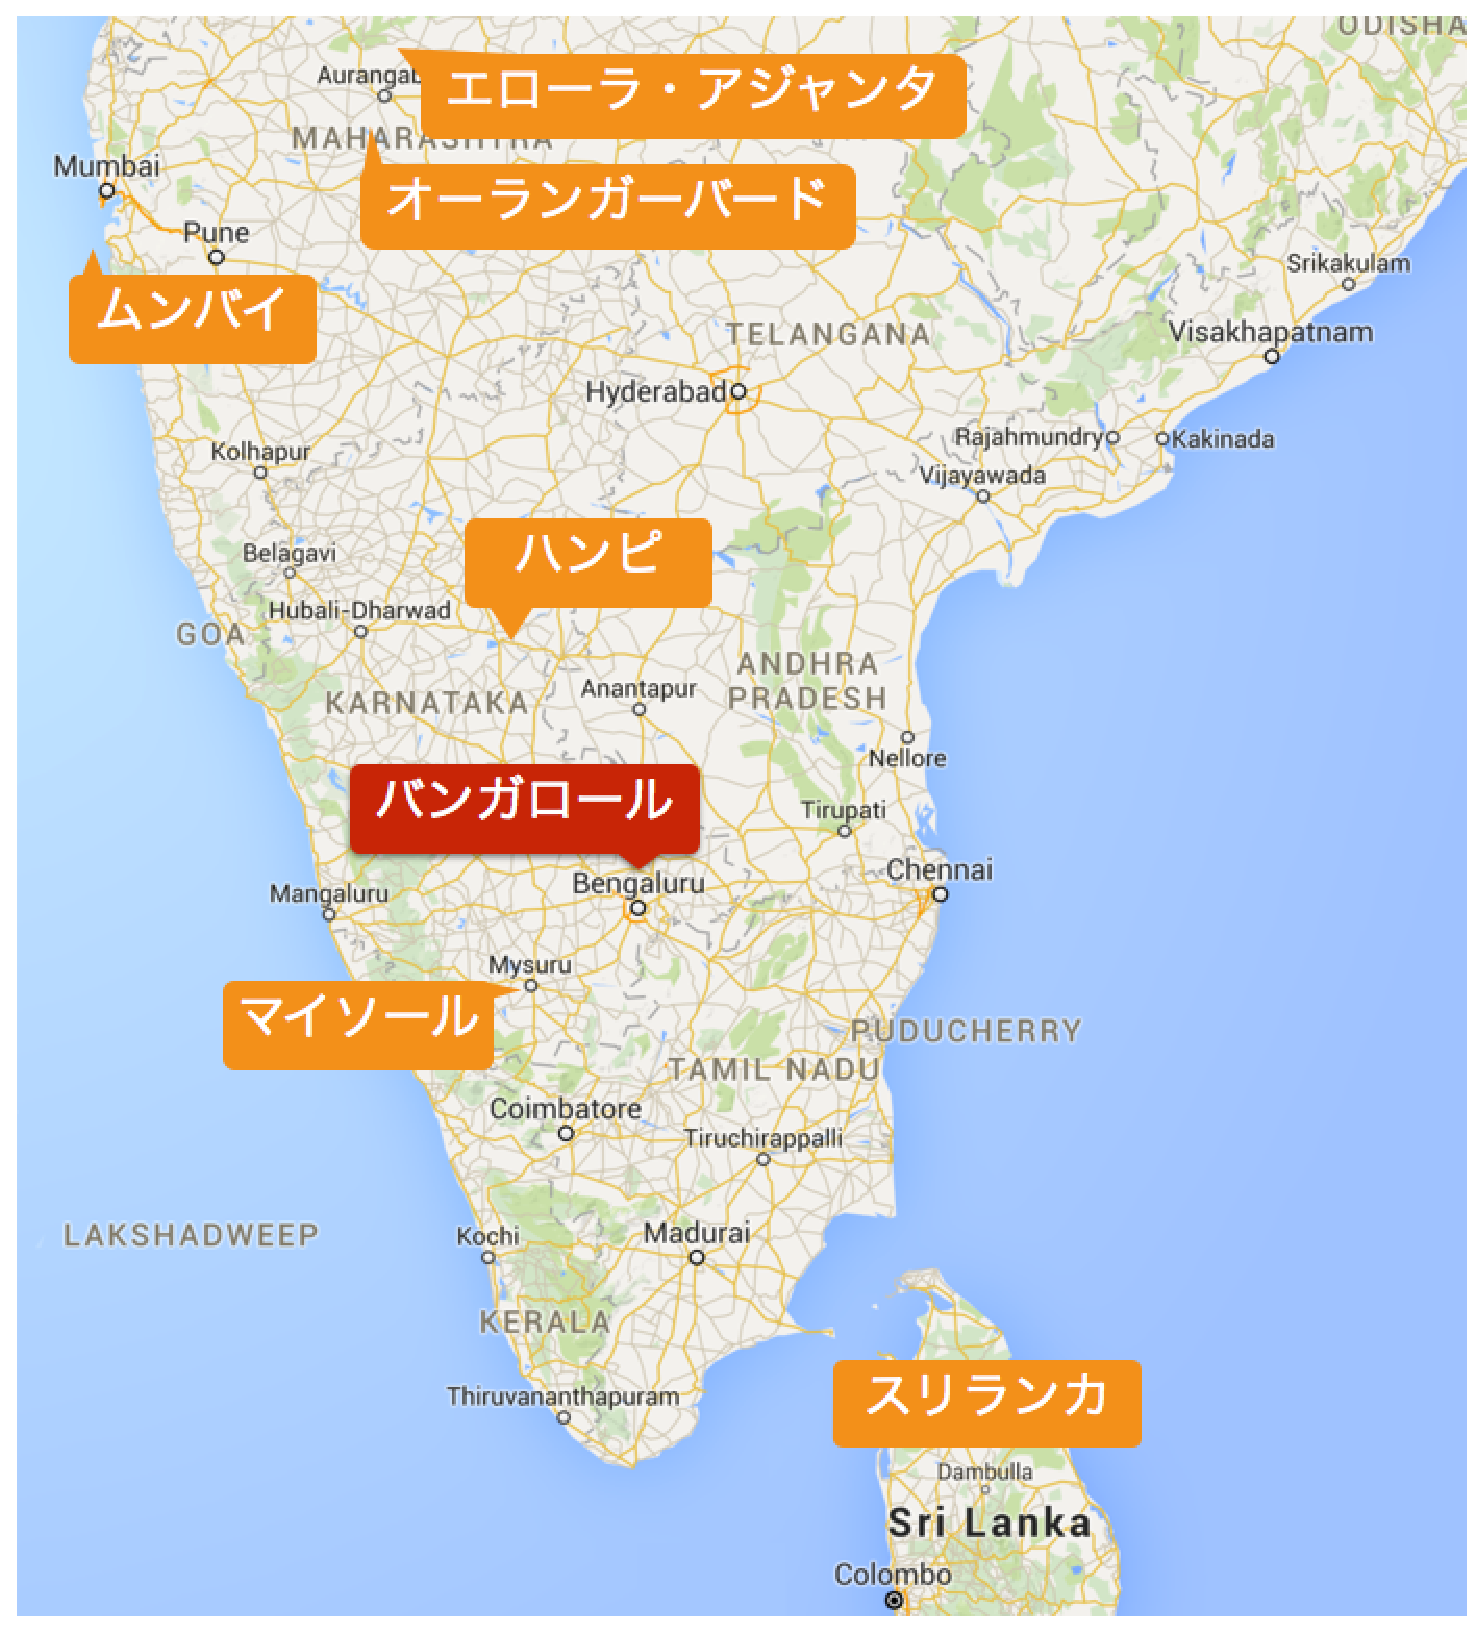
\includegraphics[width=0.9\textwidth]{pic/india.eps}
  \caption{研修期間中に訪れた南インド周辺の地域}
\end{figure}
\subsection{ムンバイ、オーランガーバード、エローラ・アジャンタ}
11月中頃にDiwaliというインドの祭典があり、それに伴い5日間の連休を取得して世界遺産に登録されているエローラ石窟群とアジャンター石窟群を訪れた。
バンガロールから飛行機でムンバイまで行き、ムンバイ市内をローカル鉄道で移動し、ムンバイからオーランガーバードまで7時間の長距離列車に乗り、
オーランガーバードからエローラとアジャンターまでは長距離バスを使った。
旅行の目的の半分以上が、インド国内の特に初めての鉄道での移動に挑戦することであった。
先述した通りインドの鉄道は乗り方が複雑なため、移動中に迷ったり乗り換えを間違えたりしても大丈夫なようにかなり余裕をもったスケジュールを組んだが、しかし実際は拍子抜けするくらい予定通りに移動ができてしまった。
ムンバイの空港から鉄道のターミナル駅に行く途中では乗り合わせた現地人が付き添って乗り換えの仕方まで教えてくれた。
特にそれでチップを求められるわけでもなかった。
オーランガーバードへ向かう長距離列車では互いに口の訊けない子連れの夫婦と相席になり、長距離バスでは高校生達と連絡先を交換し、
アジャンターで一泊したときはたまたま知り合った現地の人に家と街を案内してもらい、
そのほか行く先々でたくさんの現地の人との出会いがあってその度に何かと助けてもらった。
\begin{figure}[H]
  \begin{minipage}{0.5\hsize}
  \begin{center}
    \includegraphics[width=\textwidth]{pic/cst.eps}
  \end{center}
  \caption{ムンバイの世界遺産であり現役ターミナル駅のChhatrapati Shivaji Terminus}
  \end{minipage}
  \begin{minipage}{0.5\hsize}
  \begin{center}
    \includegraphics[width=\textwidth]{pic/mumbaitrain.eps}
  \end{center}
  \caption{ムンバイ市内の鉄道。走行中も開きっぱなしのドアから身を乗り出している人が多い。}
  \end{minipage}
\end{figure}
\begin{figure}[H]
  \begin{minipage}{0.5\hsize}
  \begin{center}
    \includegraphics[width=\textwidth]{pic/auranbus.eps}
  \end{center}
  \caption{オーランガーバードのバスターミナル。世界的な遺跡への拠点なのに英語の案内がない。}
  \end{minipage}
  \begin{minipage}{0.5\hsize}
  \begin{center}
    \includegraphics[width=\textwidth]{pic/uso.eps}
  \end{center}
  \caption{タージマハルによく似たBibi Ka Maqbara。行く先々で現地人に写真をせがまれる。}
  \end{minipage}
\end{figure}
\begin{figure}[H]
  \begin{minipage}{0.39\hsize}
  \begin{center}
    \includegraphics[width=\textwidth]{pic/diwalipic.eps}
  \end{center}
  \caption{Diwali期間中に民家の玄関口に描かれる装飾}
  \end{minipage}
  \begin{minipage}{0.39\hsize}
  \begin{center}
    \includegraphics[width=\textwidth]{pic/shonen.eps}
  \end{center}
  \caption{アジャンター石窟群に隣接する街Fardapurを案内してくれた青年}
  \end{minipage}
  \begin{minipage}{0.19\hsize}
  \begin{center}
    \includegraphics[width=\textwidth]{pic/furadapura.eps}
  \end{center}
  \caption{Fardapur青年の家と家族}
  \end{minipage}
\end{figure}
\begin{figure}[H]
  \begin{minipage}{0.5\hsize}
  \begin{center}
    \includegraphics[width=\textwidth]{pic/kago.eps}
  \end{center}
  \caption{アジャンター石窟群での「椅子」客待ち}
  \end{minipage}
  \begin{minipage}{0.5\hsize}
  \begin{center}
    \includegraphics[width=\textwidth]{pic/vendor.eps}
  \end{center}
  \caption{駅に止まるたびに売り子がやってくる}
  \end{minipage}
\end{figure}
\subsection{マイソール}
マイソールはかつてマイソール王国の首都として栄えた文化的歴史がある都市である。
バンガロールから日帰りで片道約3時間かけて鉄道で移動し、マイソール宮殿やマーケットを見て歩いた。
マーケットでは大量の生花、野菜、果物(ほとんどバナナ)、粉、布、香辛料、茶、葉っぱ、草、人の髪などが取引されており、
何のためにどうやって使うのかが分からないものが多かった。
\begin{figure}[H]
  \begin{minipage}{0.5\hsize}
  \begin{center}
    \includegraphics[width=\textwidth]{pic/market.eps}
  \end{center}
  \caption{マイソールのDevaraja Market}
  \end{minipage}
  \begin{minipage}{0.5\hsize}
  \begin{center}
    \includegraphics[width=\textwidth]{pic/kona.eps}
  \end{center}
  \caption{DiwaliやHoliの祭典で使われる粉}
  \end{minipage}
\end{figure}
\subsection{ハンピ}
ハンピはカルナータカ州北部にある都市遺跡である。
あまり観光地されておらず、中心部であってもごく小さなバザールや安宿街があるだけのとても静かな場所であった。
バンガロールからは約8時間の寝台列車でホスペットまで移動し、そこから約1時間のバスで行くことができる。
観光客にはインド人のほか欧米人が多かった。
訪れた時期が3月下旬でちょうどインドの祭典Holiの時期だったため、顔や体にカラフルな粉や液体をかけた(かけられた)人をたくさん見た。
バザールを歩いていて突然筆者のすぐ後ろで現地の子供に色水をかけられた観光客がいたが、筆者は防水対策をしていなかったためすぐに逃げた。
ハンピには広い範囲に遺跡が点在していて、地域全体に奇妙な形の岩が奇妙な構成で積み上げられている。
人工物なのか自然現象の結果なのか分からないものが多く、
いったい何がどうなればあのような岩の構成物ができるのか全く理解できなかった。
\begin{figure}[H]
  \begin{minipage}{0.5\hsize}
  \begin{center}
    \includegraphics[width=\textwidth]{pic/rock1.eps}
  \end{center}
  \caption{ハンピで唯一遺跡にならずに現役で活動し続ける寺院Virupaksha Temple}
  \end{minipage}
  \begin{minipage}{0.5\hsize}
  \begin{center}
    \includegraphics[width=\textwidth]{pic/hill.eps}
  \end{center}
  \caption{Matanga Hillからの風景。ここで昼寝した。}
  \end{minipage}
\end{figure}
\begin{figure}[H]
  \begin{minipage}{0.5\hsize}
  \begin{center}
    \includegraphics[width=\textwidth]{pic/hampipp.eps}
  \end{center}
  \caption{遺跡でピクニックをするインド人}
  \end{minipage}
  \begin{minipage}{0.5\hsize}
  \begin{center}
    \includegraphics[width=\textwidth]{pic/hampi.eps}
  \end{center}
  \caption{喜んで写真に応じてくれるが一回Rs.100}
  \end{minipage}
\end{figure}
\begin{figure}[H]
  \begin{minipage}{0.5\hsize}
  \begin{center}
    \includegraphics[width=\textwidth]{pic/hampi2.eps}
  \end{center}
  \caption{Holiを祝うHampiの子供}
  \end{minipage}
  \begin{minipage}{0.5\hsize}
  \begin{center}
    \includegraphics[width=\textwidth]{pic/dog.eps}
  \end{center}
  \caption{Holiされた犬}
  \end{minipage}
\end{figure}
\subsection{スリランカ}
スリランカはインドのすぐ南に位置しており、バンガロールから気軽に気軽に行くことができる。
スリランカ旅行を計画した当初はアーユルヴェーダ施設に一週間入ることを考えていたが、スリランカは初めてだったため
王道の遺跡・寺院巡りをすることとした。
バンガロールからネゴンボまでは飛行機で行き、そこから各都市への移動には鉄道と長距離バスを利用した。
スリランカの鉄道システムは\acrlong{ir}のように複雑でないので、特に予約せずとも問題なく現地でチケットを購入できる。
ちなみにインドの隣国であるにもかかわらずスリランカの空港(Bandaranaike)ではインドルピーの両替ができない。
これはインドルピーが国外持出し禁止とされているからであるが、タイ、シンガポール、マレーシアなどで
インド人の移民が多く集まる地域では両替が可能な場所が存在するらしい。
スリランカでも探せばコロンボでインドルピーを受け付けてくれる両替商があるかもしれない。
\begin{figure}[ht]
  \centering
  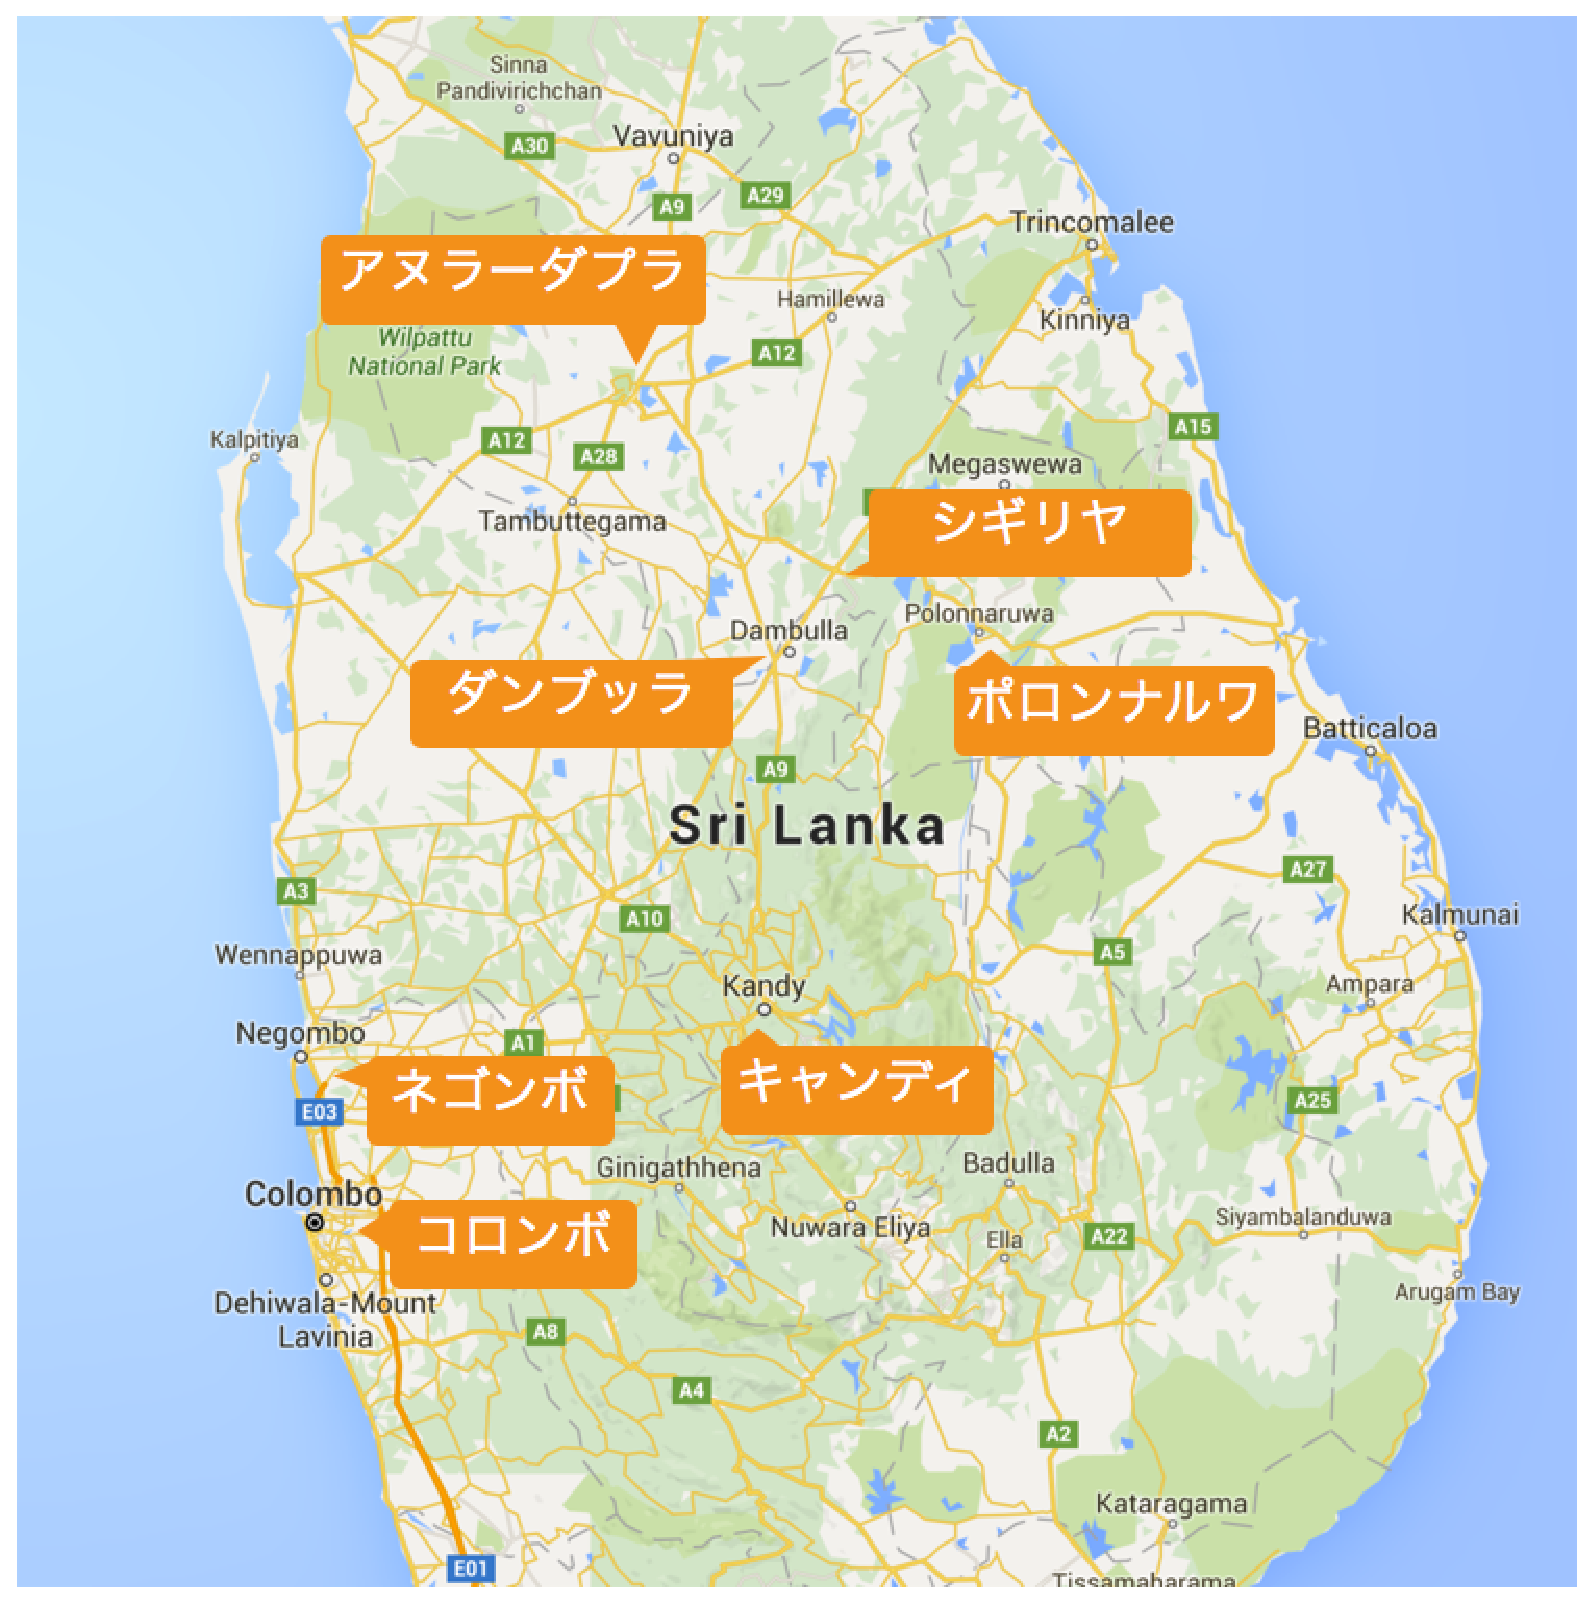
\includegraphics[width=0.9\textwidth]{pic/srilanka.eps}
  \caption{年末年始に訪れたスリランカの地域}
\end{figure}
\begin{figure}[H]
  \begin{minipage}{0.5\hsize}
  \begin{center}
    \includegraphics[width=\textwidth]{pic/fort.eps}
  \end{center}
  \caption{コロンボから各都市への起点となるFort駅}
  \end{minipage}
  \begin{minipage}{0.5\hsize}
  \begin{center}
    \includegraphics[width=\textwidth]{pic/sritrain.eps}
  \end{center}
  \caption{アヌラーダプラに到着したところ}
  \end{minipage}
\end{figure}
\begin{figure}[H]
  \begin{minipage}{0.5\hsize}
  \begin{center}
    \includegraphics[width=\textwidth]{pic/interbus.eps}
  \end{center}
  \caption{都市間を結ぶバス。本数が多くて便利。}
  \end{minipage}
  \begin{minipage}{0.5\hsize}
  \begin{center}
    \includegraphics[width=\textwidth]{pic/alpine.eps}
  \end{center}
  \caption{売りに出されているトゥクトゥク。Alpine社との関係は不明。}
  \end{minipage}
\end{figure}
\begin{figure}[H]
  \begin{minipage}{0.5\hsize}
  \begin{center}
    \includegraphics[width=\textwidth]{pic/ajinomoto.eps}
  \end{center}
  \caption{どこにでも必ず置いてあるAJINOMOTO}
  \end{minipage}
  \begin{minipage}{0.5\hsize}
  \begin{center}
    \includegraphics[width=\textwidth]{pic/monkey.eps}
  \end{center}
  \caption{ポロンナルワ遺跡群に住み着いている猿}
  \end{minipage}
\end{figure}
\begin{figure}[H]
  \begin{minipage}{0.5\hsize}
  \begin{center}
    \includegraphics[width=\textwidth]{pic/pond.eps}
  \end{center}
  \end{minipage}
  \begin{minipage}{0.5\hsize}
  \begin{center}
    \includegraphics[width=\textwidth]{pic/tooth.eps}
  \end{center}
  \end{minipage}
  \caption{キャンディ仏歯寺とその隣の池}
\end{figure}
スリランカはインドと比べると道が綺麗で、また旅行者に対して優しいという印象を持った。
現地に行っても必要な情報がきちんと英語で表示されていて、迷っていたら誰かがすぐに声をかけてくれて、かといって客引きがしつこいわけでもなく、
旅の難易度はインドよりも低いと感じた。
インドとは地理的に近く文化も似ている点が多いが、国教が仏教であるため遺跡や寺院では仏像を多く見る。
\begin{figure}[H]
  \begin{minipage}{0.33\hsize}
  \begin{center}
    \includegraphics[width=\textwidth]{pic/bicycle.eps}
  \end{center}
  \caption{ゲストハウスで借りた自転車が日本の寄付物のようで「阿倍野郵便局」と書いてあった}
  \end{minipage}
  \begin{minipage}{0.33\hsize}
  \begin{center}
    \includegraphics[width=\textwidth]{pic/sigiriya.eps}
  \end{center}
  \caption{高さ200mのシギリヤロック}
  \end{minipage}
  \begin{minipage}{0.33\hsize}
  \begin{center}
    \includegraphics[width=\textwidth]{pic/hasu.eps}
  \end{center}
  \caption{寺院の隣で売られているハスの花}
  \end{minipage}
\end{figure}
\subsection{ドイツ}
3月第一週に\acrshort{sil2linuxmp}マイルストンミーティングがドイツ・ハイデルベルグで行われた。
バンガロールからはフランクフルトまで直行便を使い、フランクフルトからハイデルベルグまでシャトルバスで移動した。
この時期のドイツはバンガロールと30℃以上の気温差があったが、インドには半袖と薄い服しか持ってこなかったためそのままの格好で行ったところ
フランクフルト空港は雪が降っていてとても寒かった。
\acrshort{sil2linuxmp}ミーティング終了後に参加者数人でハイデルベルグ城とOld Townの観光に行った際、
同行した人があまりに寒そうだと服を貸してくれた。
ハイデルベルグの古い街並みはとても美しく機能的だという印象を持った。
鉄道とトラム網がとても発達していて、道路は自転車が快適に走れるよう整備されていた。
\begin{figure}[H]
  \begin{minipage}{0.5\hsize}
  \begin{center}
    \includegraphics[width=\textwidth]{pic/tram.eps}
  \end{center}
  \caption{ハイデルベルグ街中を走るトラム}
  \end{minipage}
  \begin{minipage}{0.5\hsize}
  \begin{center}
    \includegraphics[width=\textwidth]{pic/heldel5.eps}
  \end{center}
  \caption{\acrshort{sil2linuxmp}ミーティング会場}
  \end{minipage}
\end{figure}
\begin{figure}[H]
  \begin{minipage}{0.5\hsize}
  \begin{center}
    \includegraphics[width=\textwidth]{pic/castle.eps}
  \end{center}
  \end{minipage}
  \begin{minipage}{0.5\hsize}
  \begin{center}
    \includegraphics[width=\textwidth]{pic/heldel6.eps}
  \end{center}
  \end{minipage}
  \caption{ハイデルベルグ城とそこから見下ろすOld Town}
\end{figure}
\section{食事}
インドではほとんど毎日果物を食べて生きていた。
あまり外の屋台で食べ物を買うなどのリスクを冒さなかったので、日本に帰るまで体調を崩すことはなかった。
筆者は日本では朝1リットルくらいブラックコーヒーを飲む。
しかしインドではブラックコーヒーを飲む習慣がなく、ホテルでもコーヒーはミルク入りで用意されている。
そのため毎朝ブラックコーヒーをオーダーしていた。
外国人も泊まるホテルで他にもブラックコーヒーをオーダーする人は多くいたにもかかわらず、
わざわざオーダーしないと用意してくれないシステムが改善される気配は遂になかった。
インド人は大半がベジタリアンであるため肉や魚を使ったメニューが少ない。
提供される肉も一般的な店やホテルではチキンのみである。
牛肉や豚肉を提供する店もバンガロール市内にないことはないがごく限られている。
ホテルでは毎日野菜がたっぷり朝食に並んでおり、半年間野菜と果物を主食としていたため日本にいたときよりも食生活は健康的であった。
日本でいうカレーに相当するものはあまり口にしなかった。
インド料理のことはよく分からないが、インドはカレーと一括りで言うことが失礼なほど多様なカレーのようなものがある。
むしろだいたい何を食べても固形物でも液体でもカレーのような味のするスパイスが効いているため、おそらくインドはカレーという区別がないのではないかと思う。
もちろん日本で食べるカレーの味をインドで求めるならば日本食レストランに行かなければならない。行ってもあるかどうかは分からない。
%\par
研修期間の後半になるにつれて、日本に帰ったら白米と海鮮物をとても食べたいと思うようになった。
\section{英語}
インド人の英語は聞き取りづらいというステレオタイプがあるが、発音は人それぞれである。
初めは聞き取りづらい人であっても耳が慣れれば問題なく意思疎通できるようになる。
\acrshort{hil}で働いていたインド人は英語のネイティブと遜色ないほど聞き取りやすく流暢な発音をする人が多かった。
筆者と一緒に仕事をしていたKrishnajiさん、Geetさんはそれぞれアメリカ、イギリスでの長期滞在経験があるとのことであった。
オフィスの外ではリキシャの運転手や特に地方に旅行に出かけたときに英語が通じにくいことがあった。
筆者は口頭でも文面でも結論や要点を先に伝えることを意識し、特に文法が正しくなくてもキーワードとなる単語を先に言うことを重視していた。
\par
バンガロールで耳にするまたは目にすることの多かった特徴的な英語表現としては、「営業時間」や「都合の良い時間帯」を意味するときに"timing"と言う
ことや、文中で重複を避ける際の代名詞に"the same"を使うことや、特にインド人同士の会話で"$\sim$, right ?"のようなニュアンスで"$\sim$, ノゥ ?"
と言うものがあった。
%\section{インド人}
%predictableであることがホッとする。
%時間に厳密でない。が人による。
%人を待たせることをそもそも悪いと思わない
%一番使う時間にトイレ掃除をしている
%昼のご飯を買うのに10分くらいかかる
%昼に戻ってこない。
%サービス、人が基本的に信頼できない。
%携帯電話の料金が払えない。
%電車予約システムが頻繁に落ちる。
%性悪説
\chapter*{謝辞}
\addcontentsline{toc}{chapter}{謝辞}
海外業務研修を実施するにあたり非常に多くの人に手厚いサポートをしていただきました。
派遣を推薦してくださった上長と研修を後押ししていただいた職場の皆様、
渡航前の準備から帰国後まで全面的に手続きを手伝っていただいた総務、
派遣を受け入れていただき現地の生活をサポートしてくださった\acrshort{hil}の皆様、
共に\acrshort{sil2linuxmp}プロジェクトに取り組んでいる研究所と\acrshort{hil}のメンバ、\acrshort{osadl}, \acrshort{ot}の技術者、
毎日職場まで運転してくれたドライバーと日々の生活の面倒を見てくれたホテルのスタッフ、
楽しい休日の思い出を作ってくれた日本人会テニス部と\acrshort{toast}、
旅先でフレンドリーに接してくれていろいろ助けてもらった見ず知らずの現地の人々、
非常に多くの人のサポートがあってこの業務研修ができたことを感謝しています。
今後も継続して\acrshort{sil2linuxmp}プロジェクトに取り組み、オープンソースソフトウェアの機能安全対応プロセス研究と
品質保証ノウハウ蓄積を進めます。
特に成果を\acrshort{hiics}のビジネスに展開することを念頭に置いて、引き続き\acrshort{sil2linuxmp}コミュニティと協力していく所存です。
\newline
\begin{figure}[ht]
  \centering
  \includegraphics[width=\textwidth]{pic/thanks.eps}
  \caption{\acrshort{hil}で一緒に仕事をしたチーム}
\end{figure}
